% hm-03-hermtrad.tex

\documentclass[xcolor=dvipsnames]{beamer}

\usepackage{graphicx}
% \usepackage{wrapfig}
% \usepackage{colortbl}
\usepackage{alltt}
% \definecolor{myblue}{rgb}{0.8,0.85,1}

\mode<presentation>
{
  \usetheme{Warsaw}
  \setbeamercovered{transparent}
}
% \usecolortheme[named=OliveGreen]{structure}
\setbeamertemplate{navigation symbols}{} 
\setbeamertemplate{blocks}[rounded][shadow=true] 

\newif\ifBCITCourse
\BCITCoursetrue
\BCITCoursefalse
\newif\ifWhichCourse
\WhichCoursetrue
% \WhichCoursefalse
\ifBCITCourse
\ifWhichCourse
\newcommand{\CourseName}{Statistics for Food Technology}
\newcommand{\CourseNumber}{MATH 1441}
\newcommand{\CourseInst}{BCIT}
\else
\newcommand{\CourseName}{Calculus for Geomatics}
\newcommand{\CourseNumber}{MATH 1511}
\newcommand{\CourseInst}{BCIT}
\fi
\else
\newcommand{\CourseName}{Philosophy and Literature}
\newcommand{\CourseNumber}{PHIL 375}
\newcommand{\CourseInst}{UBC}
\fi

\title{The Hermeneutic Tradition}
\subtitle{{\CourseNumber}, {\CourseInst}}

\author{\CourseName}

\date{October 17, 2017}

% \begin{frame}
%   \frametitle{iClicker Question One}
% Choose from the following options. This item will be graded.
% \begin{block}{iClicker Question}
  
% \end{block}
% \begin{description}
% \item[A\hspace{.2in}$\blacktriangleright$] 
% \item[B\hspace{.2in}$\blacktriangleright$] 
% \item[C\hspace{.2in}$\blacktriangleright$] 
% \item[D\hspace{.2in}$\blacktriangleright$] 
% \item[E\hspace{.2in}$\blacktriangleright$] 
% \item[F\hspace{.2in}$\blacktriangleright$] 
% \end{description}
% \end{frame}

% \begin{figure}[h]
% \includegraphics[scale=.3]{./extrema1.png}
% \end{figure}

\begin{document}

\begin{frame}
  \titlepage
\end{frame}

% \begin{frame}
%   \frametitle{Structuralism Table}
% \begin{figure}[h]
% 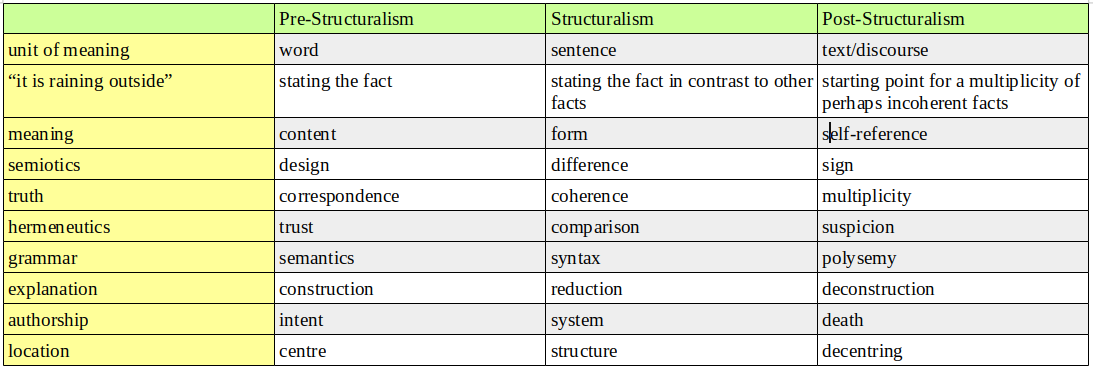
\includegraphics[scale=.3]{./structable.png}
% \end{figure}
% \end{frame}

% \begin{frame}
%   \frametitle{iClicker Question}
% Choose from the following options. This item will be graded.
% \begin{block}{iClicker Question}
% Which pain served Dostoyevsky's narrator for enjoyment?
% \end{block}
% \begin{description}
% \item[A\hspace{.2in}$\blacktriangleright$] headache
% \item[B\hspace{.2in}$\blacktriangleright$] toothache
% \item[C\hspace{.2in}$\blacktriangleright$] bellyache
% \item[D\hspace{.2in}$\blacktriangleright$] heartache
% \end{description}
% \end{frame}

% \begin{frame}
%   \frametitle{iClicker Question}
% Choose from the following options. This item will be graded.
% \begin{block}{iClicker Question}
% What is ``the most advantageous of all advantages which cannot be
% accommodated within any classification'' or calculation, according to Dostoyevsky?
% \end{block}
% \begin{description}
% \item[A\hspace{.2in}$\blacktriangleright$] religious fulfillment
% \item[B\hspace{.2in}$\blacktriangleright$] free, independent desire or will
% \item[C\hspace{.2in}$\blacktriangleright$] living in a peaceful, well-governed state
% \item[D\hspace{.2in}$\blacktriangleright$] living in mindless subservience to authority
% \end{description}
% \end{frame}

% \begin{frame}
%   \frametitle{iClicker Question}
% Choose from the following options. This item will be graded.
% \begin{block}{iClicker Question}
%   To what are humans compared in \emph{Notes from the Underground} if
%   they can be figured out by mathematical calculations?
% \end{block}
% \begin{description}
% \item[A\hspace{.2in}$\blacktriangleright$] piano keys
% \item[B\hspace{.2in}$\blacktriangleright$] thermostats
% \item[C\hspace{.2in}$\blacktriangleright$] an abacus
% \item[D\hspace{.2in}$\blacktriangleright$] seesaws
% \end{description}
% \end{frame}

% \begin{frame}
%   \frametitle{iClicker Question}
% Choose from the following options. This item will be graded.
% \begin{block}{iClicker Question}
% Complete the following excerpt by J.S. Mill: ``though the reasonings
% which connect the end or purpose with its means belong to the
% domain of science, the definition of the end itself belongs
% exclusively to {\ldots}''
% \end{block}
% \begin{description}
% \item[A\hspace{.2in}$\blacktriangleright$] Art
% \item[B\hspace{.2in}$\blacktriangleright$] Nature
% \item[C\hspace{.2in}$\blacktriangleright$] Metaphysics
% \item[D\hspace{.2in}$\blacktriangleright$] Religion
% \end{description}
% \end{frame}

% \begin{frame}
%   \frametitle{iClicker Question}
% Choose from the following options. This item will be graded.
% \begin{block}{iClicker Question}
%   How did Roger Scruton vote in the Brexit referendum?
%   % Sunday Edition 2017-10-08 second hour sundayedition_20171006_72960.mp3
% \end{block}
% \begin{description}
% \item[A\hspace{.2in}$\blacktriangleright$] he was not eligible to vote
% \item[B\hspace{.2in}$\blacktriangleright$] he voted for Brexit
% \item[C\hspace{.2in}$\blacktriangleright$] he decided not to cast a vote
% \item[D\hspace{.2in}$\blacktriangleright$] he voted against Brexit
% \end{description}
% \end{frame}

% \begin{frame}
%   \frametitle{iClicker Question}
% Choose from the following options. This item will be graded.
% \begin{block}{iClicker Question}
% Which of these examples is not addressed in the interview with Roger Scruton?
%   % Sunday Edition 2017-10-08 second hour sundayedition_20171006_72960.mp3
% \end{block}
% \begin{description}
% \item[A\hspace{.2in}$\blacktriangleright$] ISIS in Syria (religion that dehumanizes?)
% \item[B\hspace{.2in}$\blacktriangleright$] a Beethoven quartet (merely a sequence of sounds?)
% \item[C\hspace{.2in}$\blacktriangleright$] the homunculus (is there a little man in the brain?)
% \item[D\hspace{.2in}$\blacktriangleright$] Desmond, the horse (individual but not a person?)
% \end{description}
% \end{frame}

% \begin{frame}
%   \frametitle{iClicker Question}
% Choose from the following options. This item will be graded.
% \begin{block}{iClicker Question}
% What question does Nietzsche ask about Socrates?
% \end{block}
% \begin{description}
% \item[A\hspace{.2in}$\blacktriangleright$] Did he have illicit relations with Plato?
% \item[B\hspace{.2in}$\blacktriangleright$] Did he deserve his hemlock?
% \item[C\hspace{.2in}$\blacktriangleright$] Did he beat Xanthippe?
% \item[D\hspace{.2in}$\blacktriangleright$] Did he train Alexander the Great in philosophy?
% \end{description}
% \end{frame}

% \begin{frame}
%   \frametitle{iClicker Question}
% Choose from the following options. This item will be graded.
% \begin{block}{iClicker Question}
% What does Nietzsche call Kant?
% \end{block}
% \begin{description}
% \item[A\hspace{.2in}$\blacktriangleright$] that most deformed concept-cripple of all time
% \item[B\hspace{.2in}$\blacktriangleright$] the German Hume
% \item[C\hspace{.2in}$\blacktriangleright$] the great iconoclast
% \item[D\hspace{.2in}$\blacktriangleright$] the great Chinese of Hanover
% \end{description}
% \end{frame}

\begin{frame}
  \frametitle{David Hume: Of Personal Identity}
  Hume's empiricism implies his (Parfit's term) reductionist view
  of the self. Since there are no simple and constant impressions
  of the self, there also can be no such idea.
  \begin{block}{David Hume}
    He may, perhaps, perceive something simple and continued,
    which he calls \emph{himself}; though I am certain there is no
    such principle in me. But setting aside some metaphysicians of
    this kind, I may venture to affirm of the rest of mankind,
    that they are nothing but a bundle or collection of different
    perceptions, which succeed each other with an inconceivable
    rapidity, and are in a perpetual flux and movement {\ldots}
    the mind is a kind of theatre (165)
  \end{block}
Like Strawson, Hume distinguishes between identity as it regards
our thought and imagination (Strawson's ``I$^{\ast}$'') and identity
as it regards our passions and concerns (Strawson's ``I''). 
\end{frame}

\begin{frame}
  \frametitle{David Hume: Of Personal Identity}
  Cratylus and Heraclitus (see Hume's river metaphor on page 168):
  ``something unknown and mysterious, connecting the parts, beside
  their relation'' (166). At the foundation is Hume's empiricist
  psychology of ideas and impressions (percept and concept;
  perception and cognition; monism about these contrasts).
  \begin{itemize}
  \item contiguity (body-mind problem)
  \item resemblance (sympathy)
  \item causation (commonwealth or republic)
  \end{itemize}
  ``The identity, which we ascribe to the mind of man, is only a
  fictitious one'' (169). Hume thinks that the self as a
  philosophical concept is inert, and its controversies belong to
  grammar.
\end{frame}

\begin{frame}
  \frametitle{Where Am I, Or What?}
  \begin{block}{David Hume}
    Where am I, or what? From what causes do I derive my
    existence, and to what condition shall I return? Whose favour
    shall I court, and whose anger must I dread? What beings
    surround me? And on whom have I any influence, or who have
    any influence on me? I am confounded with all these questions,
    and begin to fancy myself in the most deplorable condition
    imaginable, invironed with the deepest darkness, and utterly
    deprived of the use of every member and faculty. (175)
  \end{block}
\end{frame}

\begin{frame}
  \frametitle{Why Personal Identity Isn't What Matters}
  \begin{figure}[h]
    \includegraphics[scale=0.3]{./parfit.png}
  \end{figure}
\end{frame}

\begin{frame}
  \frametitle{Derek Parfit}
  \begin{quote}
    When I believed that my existence was a further fact, I seemed
    imprisoned in myself. My life seemed like a glass tunnel, through
    which I was moving faster every year, and at the end of which
    there was darkness. When I changed my view, the walls of my glass
    tunnel disappeared. I now live in the open air. (Derek Parfit,
    Reasons and Persons, 281)
  \end{quote}
\end{frame}

\begin{frame}
  \frametitle{Questions}
  \begin{itemize}
  \item Is Nagel's view correct that it is psychologically impossible
    to believe the Reductionist View? Is Parfit's view correct that we
    can believe the truth about ourselves (280)?
  \item Do you agree with Wittgenstein that counterfactuals do not
    elucidate concepts? (``Multiverse Ethics'')
  \item What are the psychological and moral effects of the
    Reductionist View on you?
  \end{itemize}
\end{frame}

% \begin{frame}
%   \frametitle{iClicker Question}
% Choose from the following options. This item will not be graded.
% \begin{block}{iClicker Question}
% Who, according to Dilthey, was looking for an analysis of
% understanding that is at the root of the the rules we use to interpret texts?
% \end{block}
% \begin{description}
% \item[A\hspace{.2in}$\blacktriangleright$] Bertrand Russell
% \item[B\hspace{.2in}$\blacktriangleright$] Friedrich Schleiermacher
% \item[C\hspace{.2in}$\blacktriangleright$] Martin Luther
% \item[D\hspace{.2in}$\blacktriangleright$] Jacques Derrida
% \end{description}
% \end{frame}

% \begin{frame}
%   \frametitle{iClicker Question}
% Choose from the following options. This item will be graded.
% \begin{block}{iClicker Question}
% For which discipline other than the interpretation of texts is
% hermeneutics a key discipline, according to Dilthey?
% \end{block}
% \begin{description}
% \item[A\hspace{.2in}$\blacktriangleright$] history
% \item[B\hspace{.2in}$\blacktriangleright$] politics
% \item[C\hspace{.2in}$\blacktriangleright$] chemistry
% \item[D\hspace{.2in}$\blacktriangleright$] behaviourism
% \end{description}
% \end{frame}

% \begin{frame}
%   \frametitle{iClicker Question}
% Choose from the following options. This item will be graded.
% \begin{block}{iClicker Question}
%   Which of these German philosophers insists that authority is
%   accepted freely, not blindly or slavishly?
% \end{block}
% \begin{description}
% \item[A\hspace{.2in}$\blacktriangleright$] Marx
% \item[B\hspace{.2in}$\blacktriangleright$] Habermas
% \item[C\hspace{.2in}$\blacktriangleright$] Kant
% \item[D\hspace{.2in}$\blacktriangleright$] Gadamer
% \end{description}
% \end{frame}

% \begin{frame}
%   \frametitle{iClicker Question}
% Choose from the following options. This item will be graded.
% \begin{block}{iClicker Question}
% Which two examples are, according to J{\"u}rgen Habermas, examples of
% the limits of hermeneutics?
% \end{block}
% \begin{description}
% \item[A\hspace{.2in}$\blacktriangleright$] performance and rationality
% \item[B\hspace{.2in}$\blacktriangleright$] the past and the future
% \item[C\hspace{.2in}$\blacktriangleright$] psychoanalysis and critique of ideology
% \item[D\hspace{.2in}$\blacktriangleright$] the Jews and the Gnostics
% \end{description}
% \end{frame}

% \begin{frame}
%   \frametitle{iClicker Question}
% Choose from the following options. This item will be graded.
% \begin{block}{iClicker Question}
% What is Hume's comparison for the soul?
% \end{block}
% \begin{description}
% \item[A\hspace{.2in}$\blacktriangleright$] a republic or commonwealth, in which the several members are united by the reciprocal ties of government and subordination
% \item[B\hspace{.2in}$\blacktriangleright$] a prisoner of war, always treated with a respect suitable to his condition
% \item[C\hspace{.2in}$\blacktriangleright$] a commander in charge of a ship, communicating with the several parts of a vessel
% \item[D\hspace{.2in}$\blacktriangleright$] a soup, in which the ingredients are now united though they were once asunder
% \end{description}
% \end{frame}

% \begin{frame}
%   \frametitle{iClicker Question}
% Choose from the following options. This item will be graded.
% \begin{block}{iClicker Question}
% What game did Hume play to distract himself from the depressing
% conclusions of his philosophical thought?
% \end{block}
% \begin{description}
% \item[A\hspace{.2in}$\blacktriangleright$] chess
% \item[B\hspace{.2in}$\blacktriangleright$] bridge
% \item[C\hspace{.2in}$\blacktriangleright$] backgammon
% \item[D\hspace{.2in}$\blacktriangleright$] tennis
% \end{description}
% \end{frame}

\begin{frame}
  \frametitle{Hermeneutic and Scientific Method}
  \begin{equation}
    \label{eq:paumatae}
    \begin{array}{rcl}
      \mbox{understanding} & \mbox{vs.} & \mbox{explaining} \\
      \mbox{narrative} & \mbox{vs.} & \mbox{model} \\
      \mbox{inter-textuality} & \mbox{vs.} & \mbox{experiment} \\
      \mbox{coherence} & \mbox{vs.} & \mbox{falsifiability} \\
      \mbox{hypostatic} & \mbox{vs.} & \mbox{hypothetical} \\
      \mbox{texts} & \mbox{vs.} & \mbox{nature} \\
      \mbox{integration} & \mbox{vs.} & \mbox{differentiation} \\
      \mbox{dialectic} & \mbox{vs.} & \mbox{monism} \\
    \end{array}\notag
  \end{equation}
\end{frame}

\begin{frame}
  \frametitle{Structuralism}
\begin{figure}[h]
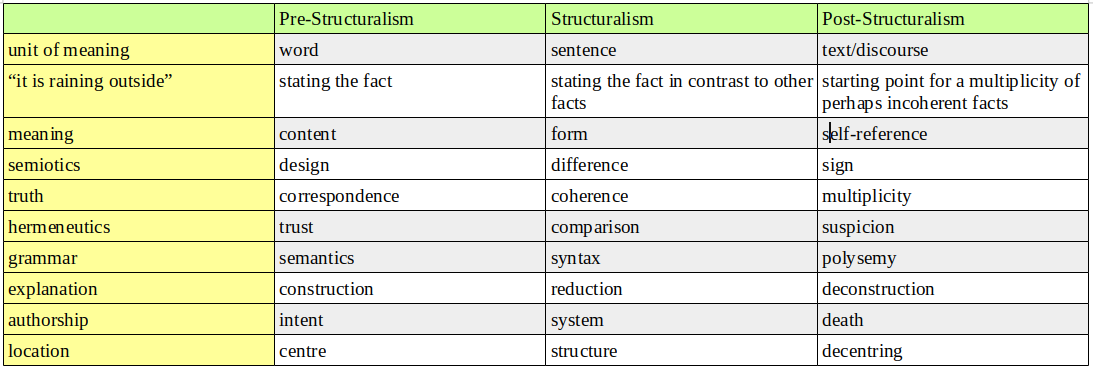
\includegraphics[scale=.3]{./structable.png}
\end{figure}
\end{frame}

\begin{frame}
  \frametitle{Wilhelm Dilthey}
  For Dilthey, there is a difference between inference from the
  particular to the general in science (objects) and in the study of
  humans (subjects). For the latter, you need to re-experience alien
  states of mind. You need to \alert{understand}, confer an inside to
  a complex of external sensory signs.
\end{frame}

\begin{frame}
  \frametitle{Wilhelm Dilthey}
  \begin{block}{Wilhelm Dilthey, page 103}
    That is indeed the immeasurable significance of literature for our
    understanding of the spiritual life and of history, for only in
    speech does the inner life of man find its fullest and most
    exhaustive, most objectively comprehensible expression. That is
    why the art of understanding centres on the exegesis or
    interpretation of those residues of human reality preserved in
    written form.
  \end{block}
\end{frame}

\begin{frame}
  \frametitle{Wilhelm Dilthey}
  The practice of exegesis (philology) leads to a conflict about the
  rules of exegesis. Hermeneutics addresses this conflict.
  \begin{itemize}
  \item interpretation and criticism of Homer
  \item Aristotle's \emph{Rhetorics} and \emph{Poetics}
  \item principle of analogy (Alexandria) versus principle of allegory
    (Pergamon, ``deliberate shrouding of pneumatic meanings in images'')
  \item between the Jews and the Gnostics: Alexandria (limits of
    allegory) and Antioch (rules of allegory)
  \end{itemize} 
\end{frame}

\begin{frame}
  \frametitle{Wilhelm Dilthey}
  \begin{itemize}
  \item Renaissance: translating alien spiritual life
  \item the \emph{Clavis} of Flacius versus Bellarmin's reliance on
    tradition
  \item Baumgarten: the historical-critical method
  \item German transcendental philosophy: creative power behind the
    contents of consciousness
  \item Ast and Schleiermacher: the hermeneutic circle 
  \end{itemize} 
\end{frame}

\begin{frame}
  \frametitle{Friedrich Schleiermacher}
  \begin{itemize}
  \item ``a genuine understanding {\ldots} can only be achieved
    through the apprehension of this systematically constructed
    whole'' (111)
  \item ``all exegesis of written works is only the systematic working
    out of that general process of understanding which stretches
    throughout our lives'' (112)
  \item there is a ``substratum of a general human nature'' (112)
  \item ``the full comprehension of the individual part already
	    presupposes comprehension of the whole'' (113)
  \item Schleiermacher's exegetical method: divisions
    $\longrightarrow$ broad outlines $\longrightarrow$ illuminate
    difficulties $\longrightarrow$ interpretation
  \item ``the ultimate goal of the hermeneutic process is to
    understand an author better than he understood himself---this is
    an idea which is the necessary consequence of the doctrine of
    unconscious creation'' (113)
  \end{itemize}
\end{frame}

\begin{frame}
  \frametitle{Wilhelm Dilthey}
  \begin{block}{Wilhelm Dilthey, page 114}
    The theory of interpretation becomes an essential connecting link
    between philosophy and the historical disciplines, an essential
    component in the foundation of the human studies themselves.
  \end{block}
\end{frame}

\begin{frame}
  \frametitle{Fields of Meaning for Hermeneutics}
  Holub lists three fields of meaning for hermeneutics in Habermas:
  \begin{enumerate}
  \item Vico-Dilthey tradition: explanation vs understanding
  \item pre-understanding: things we do not thematize as knowledge,
    which form the background or horizon for successful communication
  \item sociological bent: lifeworld
  \end{enumerate}
\end{frame}

\begin{frame}
  \frametitle{Positivism}
  Habermas uses hermeneutics in his dispute with \alert{positivism}.
  Positivism (Auguste Comte) claims that in both the natural and the
  social sciences positive (certain) knowledge comes from sensory
  experience interpreted by reason and logic. One catchy phrase of
  neopositivism, a more sophisticated version of Comte's positivism,
  is
  \begin{block}{Logical Positivism}
    The meaning of a sentence consists in its method of verification.
    (Moritz Schlick)
  \end{block}
\end{frame}

\begin{frame}
  \frametitle{Martin Heidegger}
  These are some of the changes that Heidegger initiated for
  hermeneutics:
  \begin{itemize}
  \item ``hermeneutics no longer concerns itself exclusively with the
    understanding and interpretation of written documents or speech''
    (52)
  \item ``hermeneutics takes leave of the epistemological arena and
    moves into the area of fundamental ontology'' (52)
  \item ``\emph{Dasein} may be thought of as human existence, [but] it
    should not be confused with the Cartesian or Kantian subject---it
    is that particular type of being for whom the question of Being
    arises, rather than the subject of cognition'' (52)
  \end{itemize}
\end{frame}

\begin{frame}
  \frametitle{The Hermeneutic Tradition}
\begin{figure}[h]
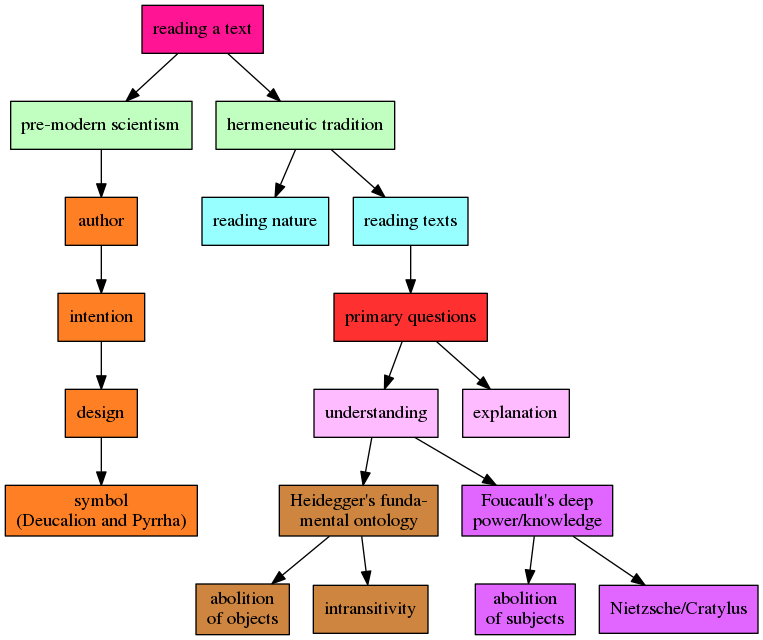
\includegraphics[scale=.32]{./subob.png}
\end{figure}
\end{frame}

\begin{frame}
  \frametitle{Martin Heidegger}
  \begin{block}{Robert Holub}
    This means that understanding is not to be conceived transitively;
    we are not concerned with understanding something. Rather,
    understanding is grasped as our way of being-in-the-world, as the
    fundamental way we exist prior to any cognition or intellectual
    activity. Ontological hermeneutics thus replaces the question of
    understanding as knowledge about the world with the question of
    being-in-the-world. (52)
  \end{block}
What does this mean for hermeneutics? For Heidegger, ``interpretation
is what we have already understood or the working out of possibilities
projected in understanding {\ldots} to understand a text in
Heidegger's sense does not involve ferreting out some meaning placed
there by the author, but the unfolding of the possibility of Being
indicated by the text'' (52).
\end{frame}

\begin{frame}
  \frametitle{Hans-Georg Gadamer}
  In \emph{Truth and Method} (note the meaning of ``and'' in Gadamer's
  title), Gadamer claims, among many other things,
  \begin{itemize}
  \item Dilthey retains the subject-object duality inherent in the
    scientific method (56)
  \item ``whereas for modern science and even for Dilthey historicity
    had been an obstacle to the ideal of objective knowledge, it was
    no [after Heidegger] transformed into a universal philosophical
    concept that enabled knowledge'' (56, compare this perhaps to
    Freud's emphasis on early childhood)
  \item Gadamer provocatively goes beyong Heidegger's fore-having,
    fore-sight, and fore-conception, to ``fore-judgment'' (prejudice)
  \item ``effective-historical consciousness''
  \item the importance of application, paradigm case legal
    hermeneutics (59)
  \end{itemize}
\end{frame}

\begin{frame}
  \frametitle{Hans-Georg Gadamer}
  \begin{block}{Robert Holub}
    Prejudice, because it belongs to historical reality itself, is not
    a hindrance to understanding but a condition for the possibility
    of understanding. Gadamer proposes a fundamental rehabilitation of
    this notion to do justice to the finitude of human existence and
    the necessarily historical mode of being-in-the-world. (57)
  \end{block}
  \begin{block}{Robert Holub}
    {\ldots} authority as embodied in individuals is not the
    consequence of subjugation, but of a recognition that the person
    in authority has superior insight and judgment. Submission to
    authority is therefore grounded in reason and freedom, not power
    and arbitrariness (60)
  \end{block}
\end{frame}

\begin{frame}
  \frametitle{Habermas and Gadamer: Areas of Agreement}
  Habermas and Gadamer share that they both oppose various forms of
  objectivism. In terms of hermeneutics, ``meaning is not something
  that can be reconstructed by empathy or by the historicist method of
  recreating the original context. Meaning is conceived as a
  sedimentation of significations that continually emerge and change
  in the course of tradition'' (63). Habermas and Gadamer also agree
  on the reintroduction of application to hermeneutics.
\end{frame}

\begin{frame}
  \frametitle{Habermas and Gadamer: Areas of Disagreement}
Habermas does not share with Gadamer the latter's rigid dichotomy of
truth and method.
\begin{block}{Robert Holub}
  Habermas's more serious objections concern the implications of
  Gadamer's work for an emancipatory political practice. At the centre
  of his critique are Gadamer's anti-Enlightenment polemics on
  prejudice, authority, and tradition. (65)
\end{block}
Habermas is missing in Gadamer the possibility for
\emph{Ideologiekritik}, the criticism of ideology. This aligns with
the problem for narrativists to make self-constituting narratives
vulnerable to evaluation. Habermas sees in Gadamer a representative of
the \alert{linguistic turn}: ``tradition is conceived not as a body of
knowledge that we master, but as a transmitted language in which we
live'' (66).
\end{frame}

\begin{frame}
  \frametitle{Gadamer's Response to Habermas's Criticism}
  \begin{block}{Robert Holub}
    Gadamer correctly understood Habermas's objection as a challenge
    to his thesis of hermeneutic universality. When Habermas calls on
    reflection to correct false ideology or when he includes labour
    and domination in a triad with language, he is in effect asserting
    that we can call on some non-hermeneutic power to determine
    meaning or have recourse to a non-hermeneutic realm to analyze
    social action. Accordingly Gadamer's defence centres on a
    reaffirmation of our embeddedness in linguistic understanding.
  \end{block}
\end{frame}

\begin{frame}
  \frametitle{Four Achievements for the Hermeneutic Method}
  \begin{enumerate}
  \item In the social sciences and humanities hermeneutic has
    contributed to a recognition that the objectivist models of the
    natural sciences are inadequate and distorting.
  \item With respect to methods in the humanities hermeneutics reminds
    us of the symbolic pre-structuring of the object that underlies
    all social inquiry and testing. 
  \item In the natural sciences it has taught us that research
    decisions are never made on exclusively scientific principles, but
    on the basis of meta-theoretical discussions in a scientific
    community. 
  \item Finally, hermeneutics provides the theoretical foundation for
    translating scientific knowledge into the normal language of the
    lifeworld. (69)
  \end{enumerate}
\end{frame}

\begin{frame}
  \frametitle{Limits of Hermeneutics}
  Two non-trivial examples of the limits of hermeneutics:
  psychoanalysis and the critique of ideology (70). ``Two of the
  checks Habermas suggests against false consensus are psychoanalysis,
  which would identify distortions caused by repressions, and the
  critique of ideology, which would decipher utterances informed by
  oppression'' (72).

  \bigskip

  Gadamer's response: revolutionary positions are included in an
  all-encompassing notion of hermeneutics (compare this view to
  Schechtman's defence of narrative self-constitution); and the
  psychoanalytic relationship with the therapist depends on authority.
\end{frame}

\begin{frame}
  \frametitle{Paul Ricoeur}
  \alert{Hermeneutics of the sacred} (Bultmann, Gadamer), where
  demythologizing is not meant to discredit symbols, but to recover
  original meaning (75). \alert{Hermeneutics of suspicion} (Marx,
  Nietzsche, Freud), which is not concerned with recovering the
  object, but with tearing away masks, with disclosing disguises, with
  revealing false consciousness (76).
  \begin{block}{Robert Holub}
    What is implicitly questioned in Habermas's objections is the
    legitimacy of carving out a privileged ontological realm that
    controls and oversees understanding. In this regard Habermas
    continues a critical tradition that rejects first philosophies for
    socially situated and pragmatically informed theory. (77)
  \end{block}
\end{frame}

\begin{frame}
  \frametitle{Notes from the Underground}
  I, for instance, would not be in the least surprised if all of a
  sudden, a propos of nothing, in the midst of general prosperity a
  gentleman with an ignoble, or rather with a reactionary and
  ironical, countenance were to arise and, putting his arms akimbo,
  say to us all: ``I say, gentleman, hadn't we better kick over the
  whole show and scatter rationalism to the winds, simply to send
  these logarithms to the devil, and to enable us to live once more at
  our own sweet foolish will!'' That again would not matter, but what
  is annoying is that he would be sure to find followers---such is the
  nature of man. And all that for the most foolish reason, which, one
  would think, was hardly worth mentioning: that is, that man
  everywhere and at all times, whoever he may be, has preferred to act
  as he chose and not in the least as his reason and advantage
  dictated. (23)
\end{frame}

\begin{frame}
  \frametitle{Notes from the Underground}
  The programme:
  \begin{itemize}
  \item I'm a sick man
  \item I'm a spiteful man
  \item I'm an unattractive man
  \end{itemize}
There are two cultural movements that NftU addresses critically: the
Enlightenment and the concluding 19th century's faith in scientific
progress. 
\end{frame}

\begin{frame}
  \frametitle{Notes from the Underground}
  Here are some concepts resisted by NftU.
  \begin{itemize}
  \item homo economicus (4)
  \item the ``men of action'' (6, 16), Rousseau's \emph{l'homme de la
      nature et de la v{\'e}rit{\'e}}, the \emph{Ch{\^a}teau Lafite}
    (18)
  \item agency (vs inertia, 34) and moral responsibility (vs massive
    innocence, page 8, ``I'm blamed when innocent''; page 12, ``you're
    in no way to blame''; page 15, ``I couldn't even blame the laws of
    nature''; page 17, ``no one is to blame'')
  \item simple, straightforward justice (10)
  \end{itemize}
\end{frame}

\begin{frame}
  \frametitle{Notes from the Underground}
  Here are some concepts resisted by NftU.
  \begin{itemize}
  \item a scientific approach to morality (12), see Sam Harris's 2011
    book \emph{The Moral Landscape: How Science Can Determine Human
      Values} (20, 22), the ``formula for all desires and caprices''
    (24)
  \item transitivity (13, 17) and objectivity
  \item the association of virtue and happiness (19)
  \item utilitarianism (19)
  \item Buckle doctrine: civilization softens man (21)
  \end{itemize}
\end{frame}

\begin{frame}
  \frametitle{Dostoyevsky's Toothache}
  \begin{quote}
    In consequence again of those accursed laws of consciousness,
    anger in me is subject to chemical disintegration. You look
    into it, the object flies off into air, your reasons
    evaporate, the criminal is not to be found, the wrong becomes
    not a wrong but a phantom, something like the toothache, for
    which no one is to blame, and consequently there is only the
    same outlet left again---that is, to beat the wall as hard as
    you can.
  \end{quote}
\end{frame}

\begin{frame}
  \frametitle{Dostoyevsky's Toothache}
  \begin{quote}
    So you give it up with a wave of the hand because you have not
    found a fundamental cause. And try letting yourself be carried
    away by your feelings, blindly, without reflection, without a
    primary cause, repelling consciousness at least for a time;
    hate or love, if only not to sit with your hands folded. The
    day after tomorrow, at the latest, you will begin despising
    yourself for having knowingly deceived yourself. Result: a
    soap-bubble and inertia. (23f)
  \end{quote}
\end{frame}

\begin{frame}
  \frametitle{Notes from the Underground}
  \begin{block}{Fyodor Dostoyevsky}
    One's own free unfettered choice, one's own caprice, however wild
    it may be, one's own fancy worked up at times to frenzy---is that
    very ``most advantageous advantage'' which we have overlooked, which
    comes under no classification and against which all systems and
    theories are continually being shattered to atoms. And how do
    these wiseacres know that man wants a normal, a virtuous choice?
    What has made them conceive that man must want a rationally
    advantageous choice? What man wants is simply independent choice,
    whatever that independence may cost and wherever it may lead. (24)
  \end{block}
\end{frame}

\begin{frame}
  \frametitle{Themes in ``Notes from the Underground'' I}
  \begin{itemize}
  \item begins with pathology and epistemological crisis
  \item intransitivity (3, 18, 23)
  \item consciousness (7, 22)
  \item Der Mann ohne Eigenschaften (a characterless creature) (5)
  \item sublime versus wretched
  \item my most normal condition and not in the least disease or
    depravity (8)
  \end{itemize}
\end{frame}

\begin{frame}
  \frametitle{Themes in ``Notes from the Underground'' II}
  \begin{itemize}
  \item enjoyment from degradation (9) why?
  \item the fundamental laws of consciousness (9)
  \item agency: direct persons and men of action (22) versus ``not
    only unable to change but could do absolutely nothing'' (9);
    the sluggard (25)
  \item the lap of nature vs. the retort (13)
  \item science (13, 15)
  \item mauvaise foi (24)
  \end{itemize}
\end{frame}

\begin{frame}
  \frametitle{Blaise Pascal}
  \begin{quote}
    When I see the blind and wretched state of men, when I survey
    the whole universe in its deadness, and man left to himself
    with no light, as though lost in this corner of the universe
    without knowing who put him there, what he has to do, or what
    will become of him when he dies, incapable of knowing
    anything, I am moved to terror, like a man transported in his
    sleep to some terrifying desert island, who wakes up quite
    lost, with no means of escape.
  \end{quote}
\end{frame}

\begin{frame}
  \frametitle{Blaise Pascal}
  \begin{quote}
    Then I marvel that so wretched a state does not drive people
    to despair {\ldots} Man's greatness comes from knowing he is
    wretched: a tree does not know it is wretched. Thus it is
    wretched to know that one is wretched, but there is greatness
    in knowing one is wretched. (Pascal, Pens{\'e}es, 114)
  \end{quote}
\end{frame}

\begin{frame}
  \frametitle{John Stuart Mill: On the Logic of the Moral Sciences}
  Are the thoughts, feelings, and actions of sentient beings a subject
  of science? Examples:
  \begin{itemize}
  \item meteorology
  \item tidology
  \item astronomy
  \item science of human nature
  \end{itemize}
Compare this to Karl Popper's idea of clouds and clocks (are all
clouds clocks? are all clocks clouds?). The criterion (for Popper, the
problem of demarcation) is prediction.
\end{frame}

\begin{frame}
  \frametitle{Art vs Science}
  The imperative mood is the characteristic of art, as distinguished
  from science. Judge vs legislator. ``The art proposes to itself an
  end to be attained, defines the end, and hands it over to science''
  $\longrightarrow$ constantly referring back to the principles of
  speculative science!
  \begin{block}{John Stuart Mill}
    Every art consists of truths of science, arranged in the order
    suitable for some practical purpose.
  \end{block}
``The definition of the end itself belongs exclusively to art.'' JSM
is an is-ought dualist, contra Sam Harris. The art of life has three
departments: morality, prudence, and aesthetics.
\end{frame}

\begin{frame}
  \frametitle{John Stuart Mill: On the Logic of the Moral Sciences}
  The umpire argument for a first principle of teleology.
  \begin{block}{John Stuart Mill}
    The general principle to which all rules of practice ought to
    conform, and the test by which they should be tried, is that of
    conduciveness to the happiness of mankind, or rather, of all
    sentient beings; in other words, that the promotion of happiness
    is the ultimate principle of teleology.
  \end{block}
However, on the whole more happiness will exist in the world if
feelings are cultivated which will make people in certain cases
regardless of happiness.
\end{frame}

\begin{frame}
  \frametitle{Nietzsche}
  What is truth?
  \begin{itemize}
  \item the comparison with women (43)
  \item seduction by grammar (44) (Hume)
  \item did Plato's Socrates deserve the hemlock?
  \item Plato's invention of the pure spirit and the good as such
  \item the fictions of logic
  \item nature's conformity to law -- matters of fact and matters of
    text
  \item reducing the strange to the familiar (Heidegger's analysis of
    truth as discovery) (48)
  \end{itemize}
  \begin{quote}
    {\ldots} without measuring reality against the purely invented
    world of the unconditional and self-identical, without a constant
    falsification of the world by means of numbers {\ldots}
  \end{quote}
\end{frame}

\begin{frame}
  \frametitle{Nietzsche}
  What is authorship and interpretation?
  \begin{itemize}
  \item ``but to a fiction there surely belongs an author? -- couldn't
    one answer simply: why?'' (45)
  \item rise above faith in grammar (46)
  \item existence without interpretation is nonsense (``all Dasein is
    essentially interpreting Dasein,'' 48) (Heidegger)
  \item profound aversion to reposing once and for all in any one
    total view of the world (51) (Marquard)
  \end{itemize}
\begin{quote}
  {\ldots} the entire conceptual antithesis `subject' and
  `object'---errors, nothing but errors! To renounce belief in one's
  ego, to deny one's own `reality'---what a triumph! 
\end{quote}
\end{frame}

\begin{frame}
  \frametitle{Friedrich Nietzsche: Gay Science, Section 355}
  \emph{The origin of our concept of `knowledge.'} I take this
  explanation from the street; I heard one of the common people say
  `he knew me right away'---and I asked myself: what do the people
  actually take knowledge to be? what do they want when they want
  `knowledge'?
\end{frame}

\begin{frame}
  \frametitle{Friedrich Nietzsche: Gay Science, Section 355}
  Nothing more than this: something unfamiliar is to be traced back to
  something \emph{familiar}. And we philosophers---have we really
  meant anything \emph{more} by knowledge? The familiar means what we
  are used to, so that we no longer marvel at it; the commonplace;
  some rule in which we are stuck; each and every thing that makes us
  feel at home--- and isn't our need for knowledge precisely this need
  for the familiar, the will to uncover among everything strange,
  unusual, and doubtful something which no longer unsettles us? Is it
  not the \emph{instinct of fear} that bids us to know? And isn't the
  rejoicing of the person who attains knowledge just rejoicing from a
  regained sense of security?
\end{frame}

\begin{frame}
  \frametitle{Friedrich Nietzsche: Gay Science, Section 355}
  Take the philosopher who imagined the world to be `knowm' when he
  had reduced it to the `idea'; wasn't it precisely because the `idea'
  was so familiar to him and he was so used to it? because he no
  longer feared the `idea'?---How little these men of knowledge
  demand! Just look at their principles and their solutions to the
  world riddle with this in mind!
\end{frame}

\begin{frame}
  \frametitle{Friedrich Nietzsche: Gay Science, Section 355}
  When they find something in, under, or behind things which
  unfortunately happens to be very familiar to us, such as our
  multiplication table or our logic or our willing and desiring, how
  happy they are right away! For `what is familiar is known': on this
  they agree. Even the most cautious among them assume that the
  familiar can at least be \emph{more easily known} than the strange;
  that for example sound method demands that we start from the `inner
  world,' from the `facts of consciousness,' because this world is
  \emph{more familiar to us}. Error of errors!
\end{frame}

\begin{frame}
  \frametitle{Friedrich Nietzsche: Gay Science, Section 355}
  The familiar is what we are used to, and what we are used to is the
  most difficult to `know'---that is, to view as a problem, to see as
  strange, as distant, as `outside us' {\ldots} The great certainty of
  the natural sciences in comparison with psychology and the critique
  of the elements of consciousness---with the \emph{unnatural}
  sciences, one might almost say---rests precisely on the fact that
  they take the \emph{strange} as their object, while it is nearly
  contradictory and absurd even to \emph{want} to take the not-strange
  as one's object {\ldots}
\end{frame}

\end{document}
